\chapter{Soluções eletrônicas de controle de acesso físico \label{cap:estadodaarte}}


\section{Introdução}

O controle de acesso é uma área da Segurança bastante explorada que oferece uma gama de soluções eletrônicas, principalmente utilizando biometria. Além da variedade e quantidade de soluções encontradas no mercado, existem também muitas propostas de soluções de controle de acesso de cunho cientifico, voltadas para atender a comunidade acadêmica ou para suprir as necessidades da sociedade em geral, oferecendo soluções que ainda não foram produzidas pela indústria. Este capítulo abordada algumas propostas acadêmicas de controle de acesso utilizando cartões eletrônicos de identificação, impressão digital e multibiometria; e apresenta os principais produtos eletrônicos de controle de acesso físico comercializados no mercado de segurança. 


\section{Soluções acadêmicas \label{solucoes_academicas}}
A seguir são apresentadas as soluções eletrônicas de controle de acesso, de caráter cientifico, divididas por tecnologia.



\subsection{Impressão digital}

 Sanchez~\cite{sanchez2011registro} propõe a automatização do processo de registro de frequência de estudantes nas Instituições de Ensino utilizando biometria da impressão digital. O foco da aplicação proposta por ele concentra-se no desenvolvimento de um algoritmo de processamento de digitais e na sua otimização para reduzir o custo de busca de registros. 
 Conforme o trabalho, a identificação dos discentes deve ser realizada em sala de aula, de modo que, o aluno precisa apenas inserir seu dedo em um leitor biométrico. O leitor captura a imagem da impressão digital para que o sistema identifique automaticamente a identidade do usuário e registre a sua presença em sala de aula, não havendo a necessidade de qualquer outro tipo de interação. A solução proposta foi desenvolvida utilizando o Kit de Desenvolvimento de Software (\textit{Software Development Kit} -- SDK) da empresa de tecnologia biométrica \textbf{Griaule Biometrics}. A partir do SDK o autor utilizou uma Interface de Programação de Aplicações (\textit{Application Programming Interface} -- API) que disponibiliza mecanismos para a captura da imagem de impressões digitais através de um sensor pré-configurado. 
 
 \nomenclature{SDK}{Kit de Desenvolvimento de Software (\textit{Software Development Kit})}
 
 
 Canedo \cite{canedo2003terminal} tem como objetivo a criação de um terminal biométrico de baixo custo para atender as demandas do mercado de controle de acesso e ponto por soluções que forneçam maior segurança e sejam capazes de serem integradas com sistemas já existentes. Este terminal biométrico possui um leitor de impressões digitais capacitivo, um \textit{display} de cristal líquido alfanumérico, um teclado e interfaces para atuadores e sensores. Sua principal tarefa  é enviar as digitais capturadas para um programa servidor utilizando o protocolo TCP/IP sobre uma rede Ethernet 10BaseT. O servidor recebe as imagens e submete a um \textit{software} que retorna o resultado da busca, sendo necessário um banco de dados para gerenciar usuários e impressões digitais. Além disso, O programa servidor pode gerenciar centenas de terminais biométricos. 
 O \textit{software} é baseado em SDK Griaule AFIS, um conjunto completo e abrangente de componentes para segurança pública e identificação em ambiente Internet e Web, que atende aos padrões WSQ (\textit{Wavelet Scalar Quantization}) do FBI e diversos padrões do Instituto Nacional Americano de Padrões (\textit{American National Standards Institute} -- ANSI) e do  Instituto Nacional de Padrões e Tecnologia (\textit{National Institute of Standards and Technology} -- NIST). O WSQ é o padrão de compressão de imagens formulado e utilizado pelo FBI para a digitalização de imagens de impressões digitais em escala de cinza \cite{ de2007analise}. Esse padrão adota uma quantização para a decomposição da imagem em 64 sub-bandas usando a transformada discreta de \textit{wavelet} (\textit{Discrete Wavelet Transform} -- DWT), em que as imagens são produzidas com qualidade de arquivamento e com taxas de compressão em torno de 20:1 \cite{brislawn1996fbi}.
 
 
 \nomenclature{WSQ}{\textit{Wavelet Scalar Quantization}}
 \nomenclature{ANSI}{Instituto Nacional Americano de Padrões (\textit{American National Standards Institute})}
 \nomenclature{NIST}{Instituto Nacional de Padrões e Tecnologia (\textit{National Institute of Standards and Technology})}
 \nomenclature{DWT}{Transformada Discreta de Wavelet (\textit{Discrete Wavelet Transform})}
 


Braga \textit{et al} \cite{stephanie2014control} apresentam um projeto de extensão para estudo de caso de um sistema de controle de acesso por biometria que consiste em um sistema embarcado capaz de controlar o acesso a um determinado ambiente, habilitando a entrada de pessoas somente por meio da impressão digital. O controle de acesso físico é feito por meio de uma tranca elétrica, que é acionada pelo sistema embarcado para a abertura de uma porta. A interface física com o usuário dispõe de um botão e três LEDs de sinalização. O botão deve ser pressionado sempre que o usuário desejar acesso ao ambiente controlado. Após o acionamento do botão o sensor biométrico é ativado e o LED amarelo é ligado, permanecendo assim até que o usuário insira o dedo no sensor. Se a digital do usuário for reconhecida o LED verde será ligado, caso contrário o LED vermelho será ativado. Na elaboração do sistema embarcado, foi confeccionada uma placa de circuito impresso que contém o circuito básico para receber o microcontrolador Atmega 328, os três LED's de sinalização, um botão, um circuito com relé, um circuito RS232 e o circuito de alimentação da placa.
 


 Duarte Neto \textit{et al} \cite{neto2014sistemas} apresentam um estudo de caso, no qual propõe um sistema automático de impressões digitais, utilizando um leitor biométrico ZFM-20 Adafruit, plataforma Arduino e uma aplicação Java. O programa foi implementado em Java e tem como objetivo controlar a execução das tarefas programadas no Arduino. O \textit{software} possui dois modos de operação: cadastro e identificação. O modo cadastro realiza um pré-cadastro na aplicação Java com os dados do indivíduo; no modo identificação o Arduino aguarda a leitura da impressão digital no leitor, para posterior comparação com as digitais armazenadas em sua \textit{flash}. Em ambos os modos, há notificações em um LCD ligado ao Arduino e na aplicação Java com mensagens via interface. A comunicação entre a interface Java (computador) e o sistema embarcado (\textit{hardware}), responsável pela leitura da digital, é feita via porta serial. Esse trabalho concentra-se basicamente no desenvolvimento de um \textit{software} para controlar a execução de operações do Arduino, via computador, tendo como estudo de caso a aplicação de leitura biométrica para autenticação de usuários \cite{neto2014sistemas}.


 
  Cruz \cite{cruz2013biometria} propõe o desenvolvimento de uma solução de controle de acesso para segurança residencial, através da implementação de um \textit{software} para autenticação de digitais utilizando um sensor Finger Key HamsterDx em conjunto com um SDK, de código aberto, disponibilizado gratuitamente pelo fabricante (Nitgen). Nesse trabalho foi desenvolvido uma interface de comunicação entre \textit{hardware} e \textit{software} através da manipulação do acesso a porta paralela via programação, para fazer o controle da leitura de impressões digitais no sensor. Através dessa comunicação é feita a leitura da digital e posteriormente a sua autenticação. O sistema conta ainda com um banco de dados para cadastro de usuários e suas respectivas digitais. Todo esse sistema foi desenvolvido para controlar o acesso físico de pessoas em ambientes residenciais e é conectado a uma fechadura eletrônica. A fechadura possui um controle remoto que foi conectado ao sistema pela porta paralela. Portanto, o sistema, faz a leitura e o reconhecimento da impressão digital e manipula o dispositivo (controle remoto) para controlar a fechadura eletrônica instalada na porta.


 
 Utilizando biometria e tecnologia móvel, Mocellin \textit{et al} \cite{mocellin2012trava} desenvolveram um sistema para controle de acesso utilizando um leitor de impressões digitais, um \textit{smartphone} e um aplicativo Android. O sistema é composto por três elementos: \textit{software} (estação-base), sistema embarcado e aplicação Android (celular). O \textit{software}, chamado de estação-base, foi desenvolvido em linguagem Java e tem a função de interface com o administrador do sistema, comunicando-se com o sistema embarcado para executar a leitura de digitais no sensor. O sistema embarcado, responsável pelo acionamento de uma fechadura eletrônica, utiliza um microcontrolador LPC1768, o qual comunica-se com a estação-base (computador) via transmissão de dados cabeada Ethernet, usando protocolo TCP/IP. Ao microcontrolador foi integrado um sensor biométrico ZFM-20 Adafruit para a leitura da impressão digital. Além desse componentes foi utilizado um aparelho celular com um aplicativo baseado em sistema operacional Android com a finalidade de controlar a fechadura eletrônica remotamente, via internet, e agregar maior funcionalidade ao sistema.



Arciniegas-Aguirre \textit{et al} \cite{aguirre2015biometric} apresentam o projeto e a implementação de um sistema biométrico de controle de acesso baseado na internet das coisas (\textit{Internet of Things} -- IoT) para a otimização do uso de recursos de \textit{hardware} \textit{open source}. Neste trabalho foram desenvolvidos um Cliente e um Servidor Web, em que o Cliente é o \textit{hardware} baseado em Arduino e o Servidor Web é o responsável pelo suporte ao Cliente. O módulo de \textit{hardware} é composto por um sensor biométrico GT511C3 Sparkfun; um Ethernet Shield, para conectar o \textit{hardware} ao Servidor Web; um módulo Relógio de Tempo Real (\textit{Real Time Clock} -- RTC), para obtenção de data e hora; e um relé para acionar uma fechadura eletrônica. Através de uma página eletrônica é possível cadastrar um usuário e consultar as informações de acesso enviadas pelo \textit{hardware}, as quais são armazenadas no Servidor. O funcionamento do sistema basicamente faz o cadastro, leitura e autenticação de impressões digitais no sistema embarcado e envia informações, como data e hora de acesso, para o Servidor.

\nomenclature{IoT}{Internet das Coisas (\textit{Internet of Things})}



 Cortez \textit{et al}\cite{cortez2016development} apresentam um sistema de chave biométrico microcontrolado para armários e gabinetes. O sistema foi desenvolvido juntamente com a tecnologia de Serviço de Mensagens Curtas (\textit{Short Message Service} -- SMS) para o envio de textos de controle. Neste sistema, é instalado um dispositivo de controle de acesso biométrico em um armário com fechadura eletrônica, o dispositivo é responsável pela leitura da digital dos usuários, abertura do armário e envio de mensagens de notificação para o administrador, incluindo alertas de tentativa de abertura da trava sem autorização, isto é, sempre que for detectada a leitura de uma digital não cadastrada, a fechadura eletrônica será travada e o sistema envia um SMS de alerta. O SMS contém um código automático que será usado para desbloquear a trava eletrônica. O \textit{hardware} é composto por um microcontrolador ATMEGA 644, um sensor Fingerprint ZFM-20 Adafruit, um teclado matricial para digitação do código de acesso, um módulo RTC para registro de data e hora de ocorrência dos eventos, um módulo GSM para envio de mensagens, uma fechadura eletrônica e um \textit{display} LCD 2x16 para a exibição das operações.
 
 
 \nomenclature{SMS}{Serviço de Mensagens Curtas (\textit{Short Message Service})}
 \nomenclature{GSM}{Sistema Global para Comunicações Móveis (\textit{Global System for Mobile Communications})}
 
 
 
 \subsection{Cartões e outros tipos de identificadores}

 Tecnologias como o RFID (Radiofrequency Identification) e o NFC (Near Field Communication) possibilitam o uso de cartões e outros objetos como elemento identificador, pois essas tecnologias são capazes de atribuir uma identidade única a um objeto. Portanto, são uma das alternativas eletrônicas de controle mais utilizadas devido apresentarem custo e complexidade de desenvolvimento inferiores aos da biometria.
 
 
 \nomenclature{NFC}{Comunicação por Campo de Proximidade (\textit{Near Field Communication})}
 
 Scagnolato \cite{scagnolato2005vital} apresenta um sistema para o controle de acesso de pessoas, utilizando a tecnologia iButton como chave eletrônica. O iButton é um chip armazenado em uma cápsula de metal confeccionada em aço inoxidável com funções lógicas que vão desde um simples número de série de 64 bits de RAM não volátil ou EEPROM, até um relógio em tempo real e sensor de temperatura. O sistema é composto por um \textit{software} que realiza o controle de entrada e saída de pessoas, um servidor de banco de dados e um microcontrolador. O \textit{software} foi implementado em ambiente visual Delphi e base de dados SQL, e um microcontrolador Motorola MC68HC908 é utilizado para leitura do número de série do iButton, que apresenta interface de comunicação baseado no protocolo 1-wire.
 

 Até um aparelho celular com tecnologia NFC pode ser utilizado como objeto identificador. Lima \cite{lima2013proposta} propõe um sistema de controle de acesso físico utilizando como chave digital um aparelho celular com tecnologia NFC. O trabalho envolve a elaboração de um terminal de acesso baseado em plataforma de prototipagem Arduino com leitor NFC, a criação de um aplicativo móvel Android e um Website para o gerenciamento do controle de acesso. O aparelho celular é utilizado como chave eletrônica e o aplicativo Android foi desenvolvido para enviar a identidade NFC criptografada para o leitor (Shield NFC) integrado ao Arduino.  O \textit{hardware} faz a leitura da identificação do celular do usuário, envia os dados diretamente para o servidor (aplicação web); em seguida o servidor faz a autenticação dos dados e retorna para o Arduino uma mensagem para o acionamento de uma fechadura eletrônica, caso o usuário seja autorizado.
 
 
 O controle de acesso pode ser uma medida de segurança adotada também em veículo. Garcia \cite{garcia2013sistema} apresenta uma solução de controle de acesso veicular utilizando tecnologia RFID. O autor tem como objetivo o desenvolvimento de um sistema microcontrolado baseado em plataforma mbed Compiler, a qual trata-se de Ambiente de Desenvolvimento Integrado (\textit{Integrated Development Environment} -- IDE) online. O sistema faz a leitura de etiquetas RFID com módulo leitor ID-12; registra informações para o controle de entrada e saída de veículos em estacionamentos; conecta-se a internet e comunica-se com uma aplicação web para gerenciamento de cadastros, edições e consultas de funcionários e veículos.
 
 \nomenclature{IDE}{Ambiente de Desenvolvimento Integrado (\textit{Integrated Development Environment})}
 

 \subsection{Multibiometria}

 Muitas soluções de controle de acesso fazem uso de um único tipo de biometria em seu sistema de autenticação. No entanto, existem projetos que vão além e propõem o uso de mais de uma característica biométrica no processo de autenticação.
 
 Em aplicações de controle de acesso um usuário pode ser coagido a se autenticar para permitir um acesso indevido. Desta forma, Oliveira \cite{oliveira2011api} propõem como alternativa para esse tipo de problema uma API que utiliza um processo de autenticação contínua com habilidade de empregar uma ou mais modalidades biométricas. O sistema verifica se o usuário que se identificou no início de uma aplicação de \textit{software} ainda está apto a continuar no sistema, sem interferências humanas ou paralisações do processo. Assim, foi projetada uma arquitetura multibiométrica visando a construção de sistemas biométricos de controle de acesso extensíveis, isto é, prontos para a inserção de novos sensores e características biométricas sem a necessidade de serem remodelados ou adaptados.







\section{Soluções de mercado\label{solucoes_mercado}}

A seguir são apresentas as principais soluções de controle de acesso encontradas no mercado. Todas as informações referentes a preço dos produtos citados nesta seção, bem como as médias de preço, foram calculadas com base em dados retirados do site \textit{Google Shopping} \cite{googleshopping}. Esse site oferece um serviço de busca gratuito, que permite a pesquisa de produtos para a comparação de preços entre diferentes vendedores \cite{sfetcu2014google, coombs2008google}. Além disso, os valores em questão são válidos somente para pagamentos à vista e não incluem o valor de frete.


 \subsection{Fechadura digital com senha}

 A \textbf{Yale YDR220L} é uma fechadura digital com teclado \textit{touch screen} (veja a Figura~\ref{yalerealliving}) que dispensa a necessidade de chaves e permite o acesso de usuários ao imóvel por meio de senha numérica, suportando o cadastro de até 25 senhas. Esse equipamento conta com guia de voz, travamento automático e é alimentado por baterias. Além disso, ele aceita um módulo de automação, vendido separadamente, que possibilita a expansão do número de usuários cadastrados, o gerenciamento e monitoramento da porta e dos usuários através de dispositivos móveis \cite{yalerealliving}. O custo médio da \textbf{Yale YDR220L} é de R\$ $1.215,00$ (mil duzentos e quinze reais).

  \begin{figure}[!ht]
  \begin{center}
  \caption{Fechadura digital com senha Yale YDR 220 L.}
  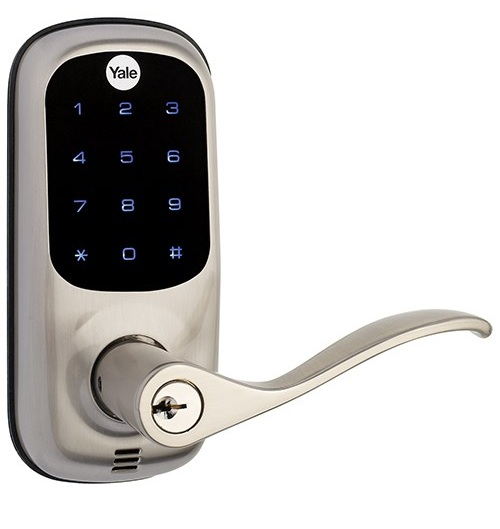
\includegraphics[scale=0.5]{figuras/cap3/yalerealliving.jpg}\\
  Fonte: Adaptado de \cite{yalerealliving}.
  \label{yalerealliving}
  \end{center}
  \end{figure}


 \subsection{Fechadura digital com senha e controle remoto}

 Além de senha, a fechadura digital \textbf{Milre Advance Control Tech 6300} (apresentada na Figura~\ref{milre6300}) pode ser controlada por controle remoto. Essa fechadura possui teclado \textit{touch screen} iluminado, dispositivo anti-hacker, travamento automático da porta, alarme contra invasão e sensor térmico interno que libera a porta em caso de incêndio. Com custo médio de R{\$} $1.183,00$ (mil cento e oitenta e três reais), a Control Tech 6300 é um modelo de embutir com maçaneta e liberação através de senha numérica ou chave digital. Esse dispositivo permite o cadastro de 8 senhas e até 45 chaves digitais, mas acompanha somente 4 chaves digitais; é alimentado com 4 pilhas tipo AA, com carga suficiente para durar até um ano, considerando uma média de utilização de vinte aberturas por dia, e emite aviso de esgotamento ao termino de carga das  pilhas \cite{milre6300}.

  \begin{figure}[!ht]
  \begin{center}
  \caption{Fechadura eletrônica Milre Advance Control Tech 6300R.}
  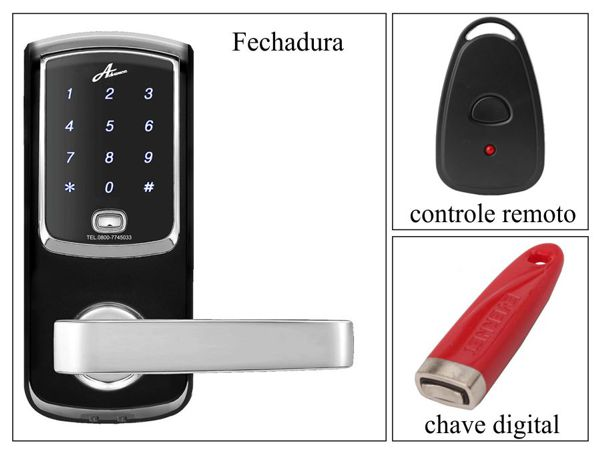
\includegraphics[scale=0.6]{figuras/cap3/milre6300.jpg}\\
  Fonte: Adaptado de \cite{milre6300}.
  \label{milre6300}
  \end{center}
  \end{figure}


 \subsection{Fechadura digital inteligente com sensor infravermelho}

 A \textbf{Samsung SHS-3321} (mostrada na Figura~\ref{samsungshs3321}) é uma fechadura digital sem maçaneta que possui leitor de cartões de $13,56$ MHz, com capacidade de registro de até setenta usuários, os quais podem obter acesso ao local protegido utilizando cartões de uso exclusivo ou códigos de segurança. Essa fechadura também dispõe de teclado numérico \textit{touch screen}; é alimentada com 4 pilhas tipo AA que duram cerca de um ano, com uma média de utilização de dez aberturas por dia; detecta a presença de possíveis intrusos por meio de sensor infravermelho; e pode ser adquirida por um valor médio de R{\$} $1.442,00$ (mil quatrocentos e quarenta e dois reais) \cite{samsungshs3321}.


  \begin{figure}[!ht]
  \begin{center}
  \caption{Fechadura inteligente Samsung SHS-3321.}
  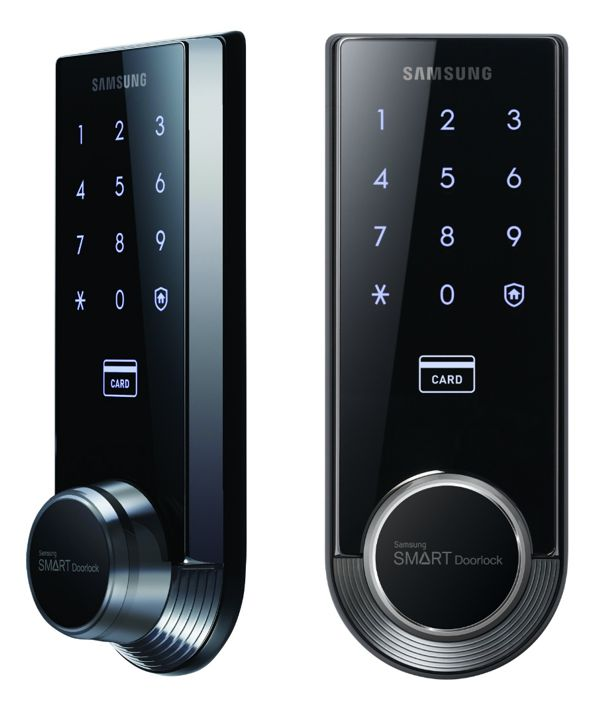
\includegraphics[scale=0.35]{figuras/cap3/samsungshs3321.jpg}\\
  Fonte: Adaptado de \cite{samsungshs3321}.
  \label{samsungshs3321}
  \end{center}
  \end{figure}


 \subsection{Fechadura biométrica com relatório de acessos}

 Utilizando biometria e senha, a \textbf{L7000} (mostrada Figura~\ref{zktecol7000}), é uma fechadura compacta que engloba múltiplas funcionalidades. Além da impressão digital e de senhas, ela permite o uso de chaves para controlar o acesso ao ambiente em que é instalada. A \textbf{L7000} possui as seguintes características: é um dispositivo com conexão USB que possibilita a troca de dados com o computador para gerar relatório utilizando o \textit{software} fornecido pelo fabricante; é capaz de armazenar 500 digitais, 100 senhas e o registro de 30.000 acessos; permite programar horários específicos de acesso para cada usuário; dispara alarme tentativa de acesso não autorizada; opera com 4 pilhas comuns (AA) que duram aproximadamente 4.000 aberturas; possui \textit{display} de diodo orgânico emissor de luz (\textit{organic light-emitting diode} -- OLED), que exibe a carga das baterias e alerta quanto a necessidade de troca \cite{zktecol7000}; e custa em média R{\$} $1.490,00$ (mil quatrocentos e noventa reais).

  \begin{figure}[!ht]
  \begin{center}
  \caption{Fechadura biométrica  ZKTeco L7000}
  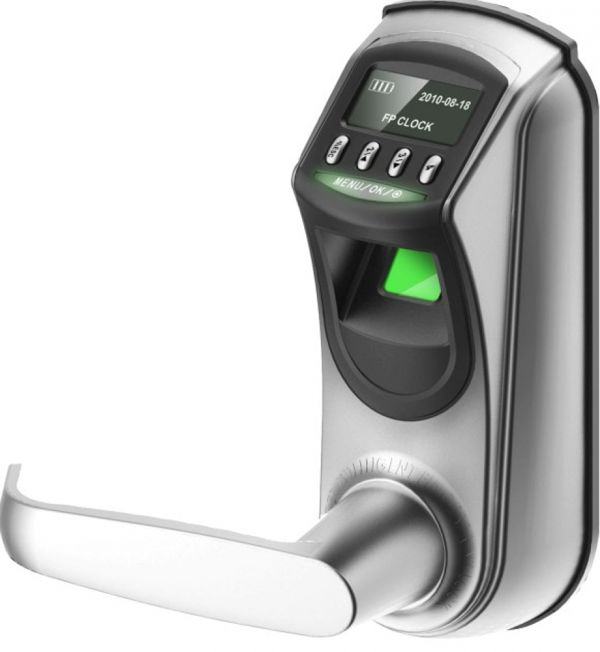
\includegraphics[scale=1]{figuras/cap3/zktecol7000.jpg}\\
  Fonte: Adaptado de \cite{zktecol7000}.
  \label{zktecol7000}
  \end{center}
  \end{figure}
  

 \subsection{Fechadura inteligente com autenticação dupla}

 Uma das mais caras opções de fechadura biométrica, a \textbf{Samsung SHS-P718} (mostrada na Figura~\ref{samsungshsp718}) pode custar até R{\$} $3.217,00$ (três mil duzentos e dezessete reais). Trata-se de um produto com design sofisticado e autenticação dupla que solicita a impressão digital e senha para abertura da porta. Tem capacidade para registrar até 100 impressões digitais, 30 usuários com senha ou cartão RFID; sua alimentação depende de 8 pilhas AA, suficientes para durarem aproximadamente um ano; inclui também sensor de movimentos infravermelho, alarme de incêndio, sons operacionais e mensagem de voz \cite{samsungshsp718}.

  \begin{figure}[!ht]
  \begin{center}
  \caption{Fechadura inteligente Samsung SHS-P718}
  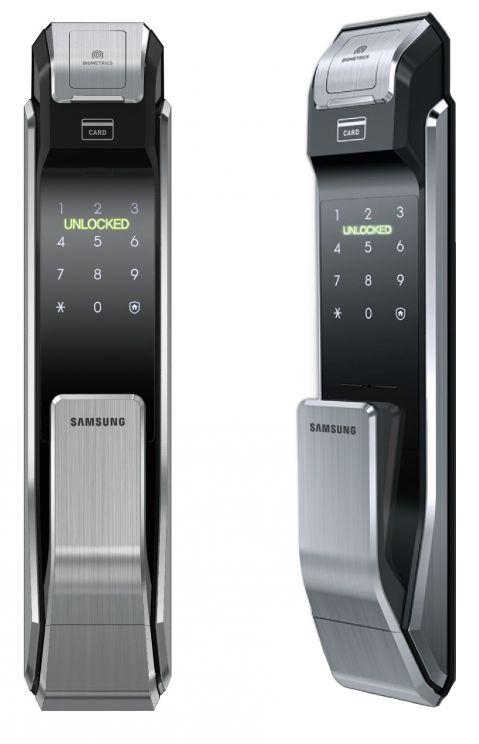
\includegraphics[scale=1.3]{figuras/cap3/samsungshsp718.jpg}\\
  Fonte: Adaptado de \cite{samsungshsp718}.
  \label{samsungshsp718}
  \end{center}
  \end{figure}


 \subsection{Controlador de acesso biométrico\label{F7}}

 O propósito de utilização do dispositivo de controle de acesso \textbf{F7} (Figura~\ref{zktecof7}), vai além de ambiente residenciais, podendo ser instalado em qualquer tipo de portaria e empresa. É um dos produtos \textit{off-line} (não depende de conexão à rede de computador), com maior capacidade de usuários. O \textbf{F7} é capaz de armazenar dados de acesso (50.000 registros) e cadastrar a impressão digital de 2.200 usuários, os quais podem utilizar a biometria, senha ou ambos. Além disso, o equipamento tem saída para sirene, sensor de porta, controle de porta, fechaduras elétricas e eletrônicas, também oferece saídas RS232, RS485 e conexão Ethernet (comunicação TCP/IP) que permite a conexão com um computador ou rede de computador para o gerenciamento dos dados armazenados, como mostra o diagrama da Figura~\ref{diagrama_zktecof7}. O aparelho é alimentado via fonte $12$ V DC e acompanha uma bateria extra que pode durar até 15 horas, dependendo do uso \cite{zktecof7}. Esse produto custa em média R{\$} $1.357,00$ (mil trezentos e cinquenta e sete reais), é distribuído por diversos fornecedores no Brasil e pode ser facilmente encontrado em lojas físicas e \textit{e-commerce}. 
 
 



  \begin{figure}[!ht]
  \begin{center}
  \caption{Controlador de acesso biométrico ZKTeco F7}
  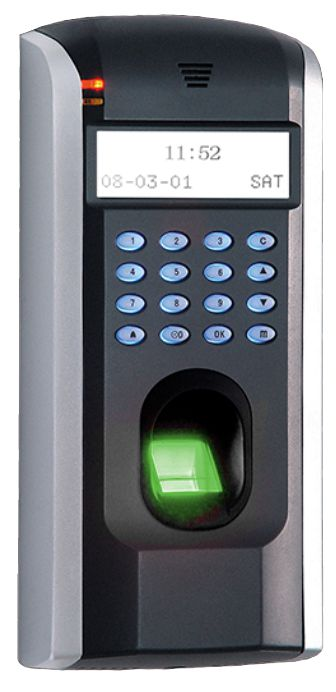
\includegraphics[scale=0.3]{figuras/cap3/zktecof7.jpg}\\
  Fonte: Adaptado de \cite{zktecof7}.
  \label{zktecof7}
  \end{center}
  \end{figure}


  \begin{figure}[!ht]
  \begin{center}
  \caption{Diagrama de conexão do controlador de acesso ZKTeco F7.}
  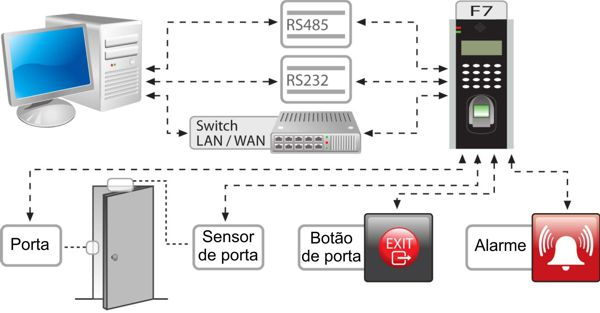
\includegraphics[scale=0.8]{figuras/cap3/diagrama_zktecof7.jpg}\\
  Fonte: Adaptado de \cite{zktecof7}.
  \label{diagrama_zktecof7}
  \end{center}
  \end{figure}


 \subsection{Controlador de acesso multifuncional}

 O controlador de acesso \textbf{iDAccess} (mostrado Figura~\ref{idaccess}), é voltado para o controle de ponto de funcionários em ambientes que possuem um grande volume de usuários. O aparelho gera relatório de acesso, faz a identificação de pessoas utilizando a impressão digital, cartão de proximidade e senha, e pode operar no modo \textit{stand alone} ou \textit{on-line}. No modo \textit{stand alone}, o equipamento é capaz de armazenar mais de 2.000 digitais e os dados de acesso podem ser consultados através de \textit{software} web embarcado. Em modo \textit{on-line}, o \textbf{iDAccess} conecta-se à rede de computador via porta Ethernet 10/100 Mbps. O dispositivo pode ser integrado a um sistema (servidor), oferecido pelo fabricante, que aumenta a sua capacidade de armazenamento para mais de 100.000 digitais e 1.000.000 de registros. Esse aparelho é alimentado por uma fonte externa de $12$ V, possui central de alarme, aceita módulo de conexão Wi-fi e GPS (opcionais). Além disso, esse sistema dispõe de serviço opcionais para monitoramento, sincronização e backup de dados em nuvem \cite{idaccess}. 

 O iDAccess se destaca pela capacidade de armazenamento de dados e registro de usuários em modo \textit{off-line}, e também pela possibilidade de expansão dessa capacidade com a integração de um sistema \textit{on-line}, além de estar na mesma faixa de preço de produtos com capacidade inferior, em média R{\$} $1.645,00$ (mil seiscentos e quarenta e cinco reais).

  \begin{figure}[!ht]
  \begin{center}
  \caption{Controlador de acesso multifuncional iDAccess.}
  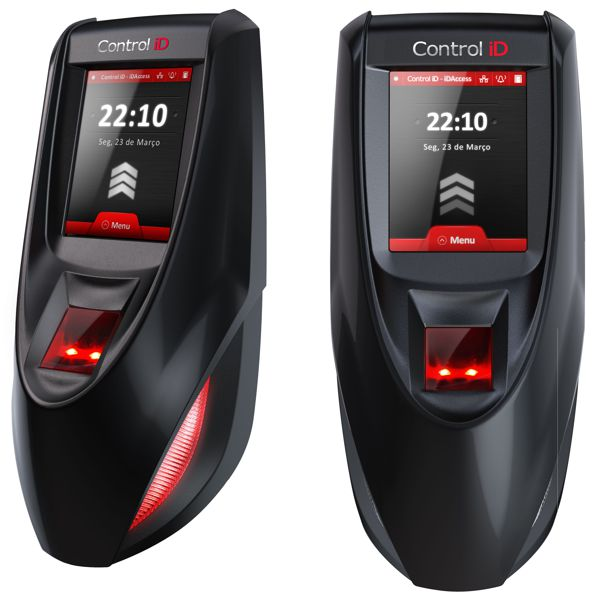
\includegraphics[scale=0.4]{figuras/cap3/idaccess.jpg}\\
  Fonte: Adaptado de \cite{idaccess}.
  \label{idaccess}
  \end{center}
  \end{figure}


 \subsection{Relógio de ponto biométrico}

 O aparelho mostrado na Figura~\ref{fingerprinttimeattendance}, conhecido apenas como \textit{Fingerprint time Attendance} em e-commerce estrangeiro ou como Relógio de Ponto Biométrico, no Brasil, é um produto chinês com poucas informações oficiais, fornecido por diferentes representantes, isto é, diferentes fabricantes produzem ou revendem um dispositivo utilizando o mesmo design, porém cada um com sua marca. No geral, esse produto é um relógio de ponto que funciona com impressão digital ou senha; tem capacidade para 600 impressões digitais e 150.000 registros, que podem ser exportados para um \textit{pen drive} em um arquivo no formato de planilha; é alimentado por fonte externa, não possui bateria \cite{fingerprinttimeattendance}; e tem um custo relativamente baixo, R{\$} 195,00 (cento e noventa e cinco reais).

  \begin{figure}[!ht]
  \begin{center}
  \caption{Relógio de ponto biométrico}
  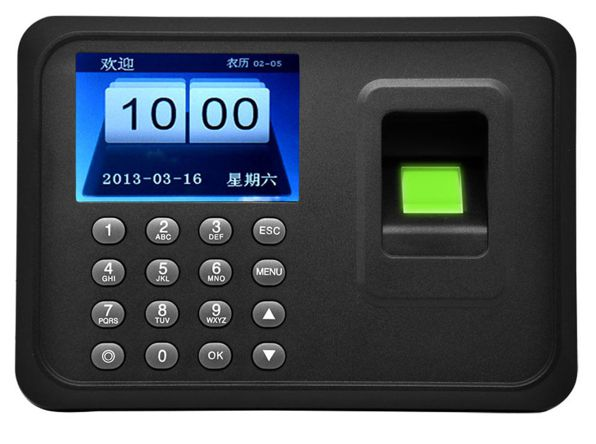
\includegraphics[scale=0.3]{figuras/cap3/fingerprinttimeattendance.jpg}\\
  Fonte: Adaptado de \cite{fingerprinttimeattendance}.
  \label{fingerprinttimeattendance}
  \end{center}
  \end{figure}
  
  
 \subsection{Leitores biométricos para sistemas de larga escala}
  
  
  \begin{figure}[!ht]
  \begin{center}
  \caption{Leitor de impressão digital U.are.U 4500}
  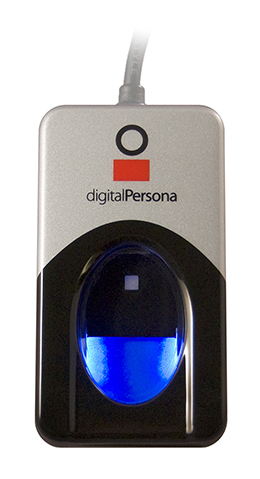
\includegraphics[scale=0.4]{figuras/cap3/uareu4500digitalpersona.jpg}\\
  Fonte: Adaptado de \cite{uareu4500digitalpersona}.
  \label{uareu4500digitalpersona}
  \end{center}
  \end{figure}
  
  
  No mercado de segurança são oferecidos uma gama de produtos eletrônicos para controle de acesso. A maioria desses produtos são fechaduras eletrônicas e relógios de ponto que utilizam tecnologia baseada em biometria. Além desse tipo de produto, existem empresas que oferecem sensores biométricos para aplicações em sistemas de larga escala, como por exemplo, o leitor de impressão digital Digital Persona U.are.U 4500\cite{uareu4500digitalpersona} (apresentado na Figura~\ref{uareu4500digitalpersona}), fabricado pela empresa Crossmatch. A Crossmatch fornece dispositivos para a empresa americana Microsoft e a brasileira Computer Digital. Esses sensores podem ser manipulados através de SDKs disponibilizados pelo fabricante ou por projetos \textit{opensource}. Também podem ser empregados em aplicações desenvolvidas pelo próprio usuário. 
  Um U.are.U 4500 pode ser adquirido por cerca de R{\$} $415,00$ (quatro centos e quinze reais) e a limitação de usuários e armazenamento de dados de acesso fica por conta das especificações do sistemas em que ele for instalado, pois essas limitações dependem de aspectos, como projeto de banco de dados, algoritmo de reconhecimento da característica biométrica e capacidade de processamento da máquina que executa o sistema.

 
 As soluções de mercado podem ser divididas em duas grandes categorias, \textit{on-line} e \textit{off-line}. As soluções de natureza \textit{on-line} normalmente custam mais caro e constituem sistemas integrados que podem reconhecer milhares de usuários, os quais podem estar situados em diferentes localizações ou pertencer a instituições distintas. Enquanto que maioria dos produtos \textit{off-line} não garantem a segurança dos dados bioméricos e registro de acesso, pois o propósito de grande parte desses produtos é o controle simples de acesso físico, sem um interesse maior no gerenciamento de dados. Essas soluções são proprietárias e o usuário não tem acesso ao dispositivo a nível de desenvolvimento, isto é, o usuário não pode fazer modificações no \textit{hardware} ou \textit{software}.


 \section{Considerações}

 O objetivo das propostas acadêmicas é oferecer soluções de controle de acesso visando o baixo custo para aplicações específicas, como o controle de frequência de alunos, controle de acesso residencial e estudos de caso, por exemplo. A maioria desses trabalhos visa beneficiar a comunidade acadêmica na qual são desenvolvidos ou a sociedade em geral, através da elaboração de projetos que atendem necessidades ainda não atendidas pela indústria. Enquanto que as soluções de mercado têm um custo de aquisição relativamente elevado e são soluções genéricas de controle de acesso que têm como objetivo oferecer mais funcionalidade, sofisticação e automatização para o usuário.
 
 
 
 